\subsection{Gtransfo\-Identity  Class Reference}
\label{class_gtransfoidentity}\index{GtransfoIdentity@{Gtransfo\-Identity}}
A do-nothing transformation. It anyway has dummy routines to mimick a GTransfo. 


{\tt \#include $<$gtransfo.h$>$}

Inheritance diagram for Gtransfo\-Identity::\begin{figure}[H]
\begin{center}
\leavevmode
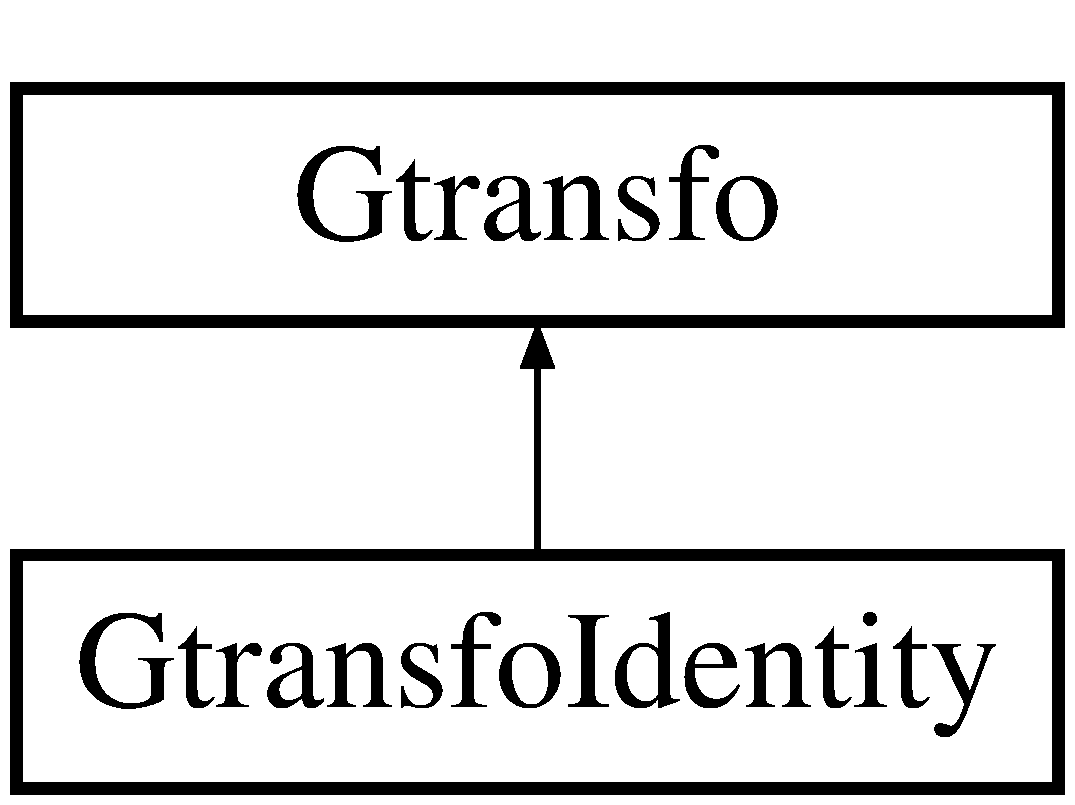
\includegraphics[height=2cm]{class_gtransfoidentity}
\end{center}
\end{figure}
\subsubsection*{Public Methods}
\begin{CompactItemize}
\item 
\index{GtransfoIdentity@{GtransfoIdentity}!GtransfoIdentity@{Gtransfo\-Identity}}\index{GtransfoIdentity@{GtransfoIdentity}!GtransfoIdentity@{Gtransfo\-Identity}}
{\bf Gtransfo\-Identity} ()\label{class_gtransfoidentity_a0}

\begin{CompactList}\small\item\em constructor.\item\end{CompactList}\item 
\index{apply@{apply}!GtransfoIdentity@{Gtransfo\-Identity}}\index{GtransfoIdentity@{GtransfoIdentity}!apply@{apply}}
void {\bf apply} (const double Xin, const double Yin, double \&Xout, double \&Yout) const\label{class_gtransfoidentity_a1}

\begin{CompactList}\small\item\em Xout = Xin; Yout = Yin !\item\end{CompactList}\item 
double {\bf fit} (const Star\-Match\-List \&List, const {\bf Gtransfo} $\ast$Prior\-Transfo=NULL, const {\bf Gtransfo} $\ast$Posterior\-Transfo=NULL)
\begin{CompactList}\small\item\em fits a transfo to a list of star pairs (p1,p2).\item\end{CompactList}\item 
\index{ReduceCompo@{ReduceCompo}!GtransfoIdentity@{Gtransfo\-Identity}}\index{GtransfoIdentity@{GtransfoIdentity}!ReduceCompo@{Reduce\-Compo}}
{\bf Gtransfo}$\ast$ {\bf Reduce\-Compo} (const {\bf Gtransfo} $\ast$Right) const\label{class_gtransfoidentity_a3}

\begin{CompactList}\small\item\em allow composition of transformations regardless of their actual types.see {\bf Gtransfo\-Compose}() {\rm (p.\,\pageref{gtransfo_h_a1})} for a user callable entry.\item\end{CompactList}\item 
\index{dump@{dump}!GtransfoIdentity@{Gtransfo\-Identity}}\index{GtransfoIdentity@{GtransfoIdentity}!dump@{dump}}
void {\bf dump} (ostream \&stream=cout) const\label{class_gtransfoidentity_a4}

\begin{CompactList}\small\item\em dumps the transfo coefficients to stream.\item\end{CompactList}\item 
\index{Npar@{Npar}!GtransfoIdentity@{Gtransfo\-Identity}}\index{GtransfoIdentity@{GtransfoIdentity}!Npar@{Npar}}
int {\bf Npar} () const\label{class_gtransfoidentity_a5}

\begin{CompactList}\small\item\em returns the number of parameters (to compute chi2's).\item\end{CompactList}\item 
\index{Clone@{Clone}!GtransfoIdentity@{Gtransfo\-Identity}}\index{GtransfoIdentity@{GtransfoIdentity}!Clone@{Clone}}
{\bf Gtransfo}$\ast$ {\bf Clone} () const\label{class_gtransfoidentity_a6}

\begin{CompactList}\small\item\em returns a copy (allocated by new) of the transformation.\item\end{CompactList}\item 
void {\bf Derivative} (const {\bf Point} \&Where, {\bf Gtransfo\-Lin} \&Derivative, const double Step=0.01) const
\begin{CompactList}\small\item\em Computes the local Derivative of a transfo. Step is used for numerical derivation.\item\end{CompactList}\item 
\index{LinearApproximation@{LinearApproximation}!GtransfoIdentity@{Gtransfo\-Identity}}\index{GtransfoIdentity@{GtransfoIdentity}!LinearApproximation@{Linear\-Approximation}}
virtual {\bf Gtransfo\-Lin} {\bf Linear\-Approximation} (const {\bf Point} \&Where, const double Step=0.01) const\label{class_gtransfoidentity_a8}

\begin{CompactList}\small\item\em linear approximation.\item\end{CompactList}\end{CompactItemize}


\subsubsection{Detailed Description}
A do-nothing transformation. It anyway has dummy routines to mimick a GTransfo.



\subsubsection{Member Function Documentation}
\index{GtransfoIdentity@{Gtransfo\-Identity}!Derivative@{Derivative}}
\index{Derivative@{Derivative}!GtransfoIdentity@{Gtransfo\-Identity}}
\paragraph{\setlength{\rightskip}{0pt plus 5cm}void Gtransfo\-Identity::Derivative (const {\bf Point} \& {\em Where}, {\bf Gtransfo\-Lin} \& {\em Derivative}, const double {\em Step} = 0.01) const\hspace{0.3cm}{\tt  [virtual]}}\hfill\label{class_gtransfoidentity_a7}


Computes the local Derivative of a transfo. Step is used for numerical derivation.

the Derivative is represented by a {\bf Gtransfo\-Lin} {\rm (p.\,\pageref{class_gtransfolin})}, in which (hopefully), the offset terms are zero. Derivative should  transform a vector of offsets into a vector of offsets. 

Reimplemented from {\bf Gtransfo} {\rm (p.\,\pageref{class_gtransfo_a9})}.\index{GtransfoIdentity@{Gtransfo\-Identity}!fit@{fit}}
\index{fit@{fit}!GtransfoIdentity@{Gtransfo\-Identity}}
\paragraph{\setlength{\rightskip}{0pt plus 5cm}double Gtransfo\-Identity::fit (const Star\-Match\-List \& {\em List}, const {\bf Gtransfo} $\ast$ {\em Prior\-Transfo} = NULL, const {\bf Gtransfo} $\ast$ {\em Posterior\-Transfo} = NULL)\hspace{0.3cm}{\tt  [inline, virtual]}}\hfill\label{class_gtransfoidentity_a2}


fits a transfo to a list of star pairs (p1,p2).

After the fit this(Prior\-Transfo(p1)) yields approximately Posterior\-Transfo(p2). The returned value is the chi2. 

Reimplemented from {\bf Gtransfo} {\rm (p.\,\pageref{class_gtransfo_a4})}.

The documentation for this class was generated from the following file:\begin{CompactItemize}
\item 
{\bf gtransfo.h}\end{CompactItemize}
